%% ----------------------------------------------------------------
%% GDP.tex
%% ---------------------------------------------------------------- 
\documentclass{.style/ecsgdp}         % Use the GDP Report Style
\graphicspath{{./Figures/}}   % Location of your graphics files
\usepackage{array}
\usepackage{listings}
\usepackage{pdflscape}
\usepackage{pgfgantt}
\usepackage{pgfplots}
\usepackage{enumitem}       % For making numbered indent lists
\usepackage{color}
\usepackage{graphicx,subfigure}
\usepackage{multirow}
\usepackage{todonotes}
\usepackage{tikz}
\usetikzlibrary{automata,positioning}
\lstset{language=C}

\hypersetup{colorlinks=true}   % Set to false for black/white printing
%%% ----------------------------------------------------------------
%% Definitions.tex
%% ---------------------------------------------------------------- 
\newcommand{\BibTeX}{{\rm B\kern-.05em{\sc i\kern-.025em b}\kern-.08em T\kern-.1667em\lower.7ex\hbox{E}\kern-.125emX}}

%% People
\newcounter{address}
\setcounter{address}{1}
\renewcommand{\theaddress}{\textsuperscript{\fnsymbol{address}}}
\newcommand{\address}[1]{\refstepcounter{address}\theaddress#1\\}
\newcommand{\Name}[3]{\texorpdfstring{\href{mailto:#3}{#2}#1}{#2}\xspace}
\newcommand{\SteveRGunn}[1]{\Name{#1}{Steve R. Gunn}{S.R.Gunn@ecs.soton.ac.uk}}

%% Dingbats
\newcommand{\tick}{\ding{51}}
\newcommand{\cross}{\ding{55}}

%% Calculus
\newcommand{\pd}[2]{\ensuremath{\frac{\partial #1}{\partial #2}}\xspace}
\newcommand{\fd}[2]{\ensuremath{\frac{d #1}{d #2}}\xspace}
\newcommand{\dint}{\ensuremath{\int\!\!\!\int}\xspace}
\newcommand{\tint}{\ensuremath{\int\!\!\!\int\!\!\!\int}\xspace}

%% Math Sets
\newcommand{\Q}[1]{\ensuremath{\mathbb{#1}}\xspace}
\newcommand{\R}{\Q{R}}

%% Matrix, Vector
\newcommand{\V}[1]{\ensuremath{\boldsymbol{#1}}\xspace}
\newcommand{\M}[1]{\ensuremath{\boldsymbol{#1}}\xspace}
\newcommand{\0}{\V{0}}
\newcommand{\1}{\V{1}}
\newcommand{\I}{\M{I}}

%% Math Functions
\newcommand{\F}[1]{\ensuremath{\mathrm{#1}}\xspace}
\newcommand{\sgn}{\F{sgn}}
\newcommand{\tr}{\F{trace}}
\newcommand{\diag}{\F{diag}}

%% Math Names
\newcommand{\N}[1]{\ensuremath{\mathit{#1}}\xspace}

%% Data
\newcommand{\mc}[1]{\ensuremath{\mathcal{#1}}\xspace}
\newcommand{\Hyp}{\mc{H}}
\newcommand{\D}{\mc{D}}

%% Kernel
\newcommand{\K}{\M{K}}
\newcommand{\eins}{\texorpdfstring{\ensuremath{\epsilon}}{\textepsilon}-insensitive\xspace}
\newcommand{\e}{\ensuremath{\epsilon}\xspace}
\newcommand{\Bxi}{\ensuremath{\boldsymbol{\xi}}\xspace}
\newcommand{\Kanova}{\ensuremath{\mathit{K_{ANOVA}}}\xspace}
\newcommand{\Kspline}{\ensuremath{\mathit{K_{spline}}}\xspace}

%% Bayesian
\newcommand{\MP}{\ensuremath{\mathit{{\scriptscriptstyle \hspace{-1.5pt}M\hspace{-1.5pt}P}}}\xspace}
\newcommand{\ML}{\ensuremath{\mathit{{\scriptscriptstyle \hspace{-1.5pt}M\hspace{-1.5pt}L}}}\xspace}
\newcommand{\Qw}{\ensuremath{Q_{\w}(\w)}\xspace}
\newcommand{\Qa}{\ensuremath{Q_{\Ba}(\Ba)}\xspace}
\newcommand{\Qb}{\ensuremath{Q_{\beta}(\beta)}\xspace}
\newcommand{\wMPab}{\ensuremath{\w_{\MP|\bar {\Ba},\bar \beta}}\xspace}
\newcommand{\wMP}{\ensuremath{\w_{\MP}}\xspace}
\newcommand{\yMP}{\ensuremath{y_{\MP}}\xspace}
\newcommand{\BaMP}{\ensuremath{\Ba_{\hspace{1pt}\MP}}\xspace}
\newcommand{\aMP}{\ensuremath{\alpha_{\hspace{1pt}\MP}}\xspace}
\newcommand{\bMP}{\ensuremath{\beta_{\hspace{1pt}\MP}}\xspace}
\newcommand{\Sab}{\ensuremath{\M{\Sigma}_{\bar \Ba,\bar \beta}}\xspace}
\newcommand{\Ba}{\ensuremath{\boldsymbol{\alpha}}\xspace}
\newcommand{\Bb}{\ensuremath{\boldsymbol{\beta}}\xspace}
\newcommand{\Bm}{\ensuremath{\boldsymbol{\mu}}\xspace}
\newcommand{\BL}{\ensuremath{\boldsymbol{\Lambda}}\xspace}
\newcommand{\BPhi}{\ensuremath{\boldsymbol{\Phi}}\xspace}
\newcommand{\SMP}{\ensuremath{\M{\Sigma}_{\MP}}\xspace}

\newcommand{\Pa}{\ensuremath{P(\alpha|\mathcal{H})}\xspace}
\newcommand{\Pb}{\ensuremath{P(\beta|\mathcal{H})}\xspace}
\newcommand{\Pab}{\ensuremath{P(\alpha,\beta|\mathcal{H})}\xspace}
\newcommand{\Pw}{\ensuremath{P(\w|\mathcal{H})}\xspace}
\newcommand{\PD}{\ensuremath{P(\D|\mathcal{H})}\xspace}
\newcommand{\PwIa}{\ensuremath{P(\w|\alpha,\mathcal{H})}\xspace}
\newcommand{\PDIwb}{\ensuremath{P(\D|\w,\beta,\mathcal{H})}\xspace}
\newcommand{\PDwab}{\ensuremath{P(\D,\w,\alpha,\beta|\mathcal{H})}\xspace}
\newcommand{\PDIw}{\ensuremath{P(\D|\w,\mathcal{H})}\xspace}
\newcommand{\PwID}{\ensuremath{P(\w|\D,\mathcal{H})}\xspace}
\newcommand{\PwabID}{\ensuremath{P(\w,\alpha,\beta|\D,\mathcal{H})}\xspace}

\newcommand{\PanH}{\ensuremath{P(\alpha)}\xspace}
\newcommand{\PbnH}{\ensuremath{P(\beta)}\xspace}
\newcommand{\PabnH}{\ensuremath{P(\alpha,\beta)}\xspace}
\newcommand{\PwnH}{\ensuremath{P(\w)}\xspace}
\newcommand{\PDnH}{\ensuremath{P(\D)}\xspace}
\newcommand{\PwIanH}{\ensuremath{P(\w|\alpha)}\xspace}
\newcommand{\PDIwbnH}{\ensuremath{P(\D|\w,\beta)}\xspace}
\newcommand{\PDwabnH}{\ensuremath{P(\D,\w,\Ba,\beta)}\xspace}
\newcommand{\PDIwnH}{\ensuremath{P(\D|\w)}\xspace}
\newcommand{\PwIDnH}{\ensuremath{P(\w|\D)}\xspace}
\newcommand{\PwabIDnH}{\ensuremath{P(\w,\alpha,\beta|\D)}\xspace}

\newcommand{\PDwBab}{\ensuremath{P(\D,\w,\Ba,\beta|\mathcal{H})}\xspace}
\newcommand{\PwIBa}{\ensuremath{P(\w|\Ba,\mathcal{H})}\xspace}
\newcommand{\PBab}{\ensuremath{P(\Ba,\beta|\mathcal{H})}\xspace}
\newcommand{\PwBabID}{\ensuremath{P(\w,\Ba,\beta|\D,\mathcal{H})}\xspace}

\newcommand{\PBanH}{\ensuremath{P(\Ba)}\xspace}
\newcommand{\PwIBanH}{\ensuremath{P(\w|\Ba)}\xspace}

%% Snakes
\newcommand{\Esnake}{\ensuremath{\mathit{E_{snake}}}\xspace}
\newcommand{\Eimage}{\ensuremath{\mathit{E_{image}}}\xspace}
\newcommand{\Econt}{\ensuremath{\mathit{E_{cont}}}\xspace}
\newcommand{\Ecurv}{\ensuremath{\mathit{E_{curv}}}\xspace}
\newcommand{\Eint}{\ensuremath{\mathit{E_{int}}}\xspace}
\newcommand{\Eext}{\ensuremath{\mathit{E_{ext}}}\xspace}
\newcommand{\Eterm}{\ensuremath{\mathit{E_{term}}}\xspace}
\newcommand{\Eline}{\ensuremath{\mathit{E_{line}}}\xspace}
\newcommand{\Eedge}{\ensuremath{\mathit{E_{edge}}}\xspace}
\newcommand{\Econ}{\ensuremath{\mathit{E_{con}}}\xspace}
\newcommand{\Eangle}{\ensuremath{\mathit{E_{angle}}}\xspace}
\newcommand{\Elshape}{\ensuremath{\mathit{E_{lshape}}}\xspace}
\newcommand{\Eedgedir}{\ensuremath{\mathit{E_{edgedir}}}\xspace}
\newcommand{\Emodel}{\ensuremath{\mathit{E_{model}}}\xspace}
\newcommand{\wte}{\ensuremath{\mathit{w_{term}}}\xspace}
\newcommand{\wli}{\ensuremath{\mathit{w_{line}}}\xspace}
\newcommand{\wed}{\ensuremath{\mathit{w_{edge}}}\xspace}
\newcommand{\wco}{\ensuremath{\mathit{w_{con}}}\xspace}

%% Environments
\newcounter{alg}
\newenvironment{algorithm}[1]
{
    \stepcounter{alg}
    \begin{table}[htb]
    \centering
    \begin{tabular}[t]{ll}
    \hline&\\
    \multicolumn{2}{l}{\bf Algorithm \arabic{alg}: #1}\\&\\
} {
    &\\
    \hline
    \end{tabular}
    \end{table}
}
            % Include your abbreviations
\newcommand{\namedsection}[2]{\section[#1]{#1 \hfill {\small \color{gray} #2}}} % Use this to create sections with authorship: \namedsection{Section Name}{Your name}
\newcommand{\namedsubsection}[2]{\subsection[#1]{#1 \hfill {\small \color{gray} #2}}} % Use this to create subsections with authorship: \namedsubsection{Section Name}{Your name}

\newcommand{\note}[1]{\todo[inline]{#1}}


%% ----------------------------------------------------------------
\begin{document}
	\frontmatter
	\title{Ultra-Low-Power Exercise Monitoring Applications for Sub-Threshold Micro-Controllers}
	\authors    {\\ \texorpdfstring
		{\href{mailto:djap1g11@ecs.soton.ac.uk}{Daniel Playle}}
		{Daniel J. A. Playle}
		\\
		\texorpdfstring
		{\href{mailto:ams2g11@ecs.soton.ac.uk}{Emily Shepherd}}
		{Emily Shepherd}
		\\
		\texorpdfstring
		{\href{mailto:mg8g12@ecs.soton.ac.uk}{Mohit Gupta}}
		{Mohit Gupta}
		\\
		\texorpdfstring
		{\href{mailto:tlf1g12@ecs.soton.ac.uk}{Toby Finch}}
		{Toby Finch}
		\\
		\texorpdfstring
		{\href{mailto:cp10g12@ecs.soton.ac.uk}{Calin Pasat}}
		{Calin Pasat}
	}
	\addresses  {\groupname\\\deptname\\\univname}
	\date       {\today}
	\subject    {}
	\keywords   {}
	\supervisor{Dr. Geoff Merrett \\ Dr. Alex Weddell}
	\examiner{Dr. Klaus-Peter Zauner}
	\degree     {Master of Engineering}
	\maketitle
	\begin{abstract}
		This work is all about \dots
	\end{abstract}
	\tableofcontents
	\listoffigures
	\listoftables
	\lstlistoflistings
	\listofsymbols{ll}
	{
		$S$ & The scale factor of a fixed-point number \\
		$B$ & The number of bits to shift a fixed-point number \\
		$L$ & A Layer in a MultiLayer Perceptron. Can be considered a set of nodes \\
		$LAYERS$ & The set of all Layers in a MultiLayer Perceptron
	}
	%\acknowledgements{Thanks to no one.}
	%\dedicatory{To \dots}
	\mainmatter
	%% ----------------------------------------------------------------
	% Introduction chapter
	\chapter{Introduction}

Ultra-Low Power Processors, such as ARM's Cortex-M0+, are becoming an increasingly appealing area of research, particularly because they provide a platform for the Internet of Things. As our culture develops new ways for technology to aid our every-day lives, the devices which support these progressions are required to be less and less intrusive, forcing companies to search for new methods of making systems smaller and require lower power, especially as ``essentially all IoT sensor nodes will be powered by small batteries and to a lesser extent by energy harvesting'' \cite{iot_power}.

However, such processors clearly create very tight constraints for potential developers, as processing power is often limited, leading to the ever-continuing requirement for more efficient and optimised algorithms. As memory usage is also proportional to power consumption, the RAM available on such systems is extremely limiting. As we begin to rely on these systems more and more, these constraints make it a growing challenge to implement systems which are not only useful, but can be relied upon to function when needed. This is particularly important in cases in which a device is being used for safety-critical operations, which is becoming increasingly common \cite{iot_saftey} \cite{iot_saftey2}.

ARM is currently investigating the concept of a sub threshold Cortex-M0+ \cite{arm_sub}, which attempts to push the extremes of these constraints further by providing just 8 kB of memory for both program code and data, and running at just a few hundred kHz. This project aims to research and develop an algorithm which is capable of running on such a device, to act as a proof of concept that such a processor would be worthwhile.

\namedsection{Project Overview}{Finch}

The particular algorithm that the group developed is a way to identify and monitor exercises performed by a human wearer. These are specifically exercises which can be done on aeroplanes to reduce the risk of suffering from Deep Vein Thrombosis, a condition where a blood clot can form in one of the deep veins in the body, most commonly the legs. This can lead to further complications such as pulmonary embolism which occurs when part of the blood clot moves and blocks a blood vessel in the lungs \cite{dvt}. Long-haul flights can increase the risk of getting DVT because of the long periods of time sitting down and not moving which reduces circulation in the legs.

\begin{figure}[h]
  \centering
    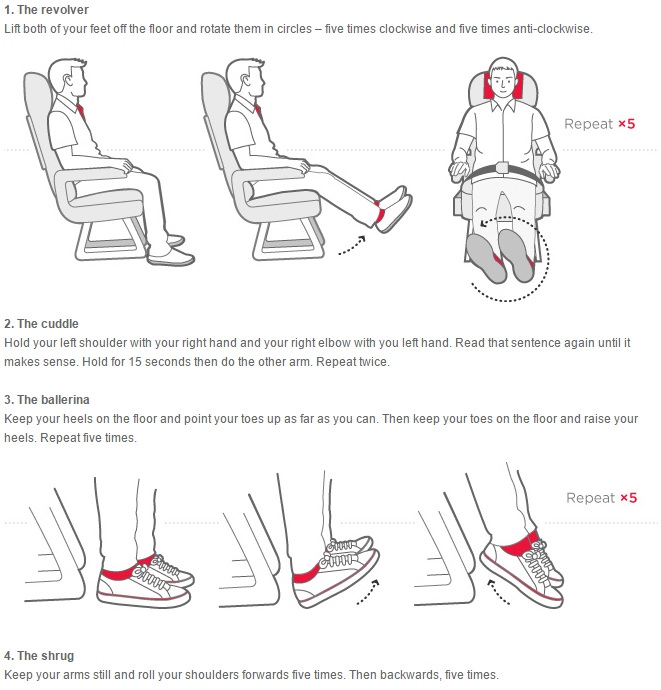
\includegraphics[width=1.0\textwidth]{figures/exercises}
  \caption{In-flight exercises \cite{virgin2015exercises}}
  \label{fig:exercises}
\end{figure}

Figure \ref{fig:exercises} shows some of the in-flight exercises which can be performed. A few of them were looked into including the revolver, the ballerina and the shrug. These involve lifting both feet off the floor and rotating them in circles in clockwise and anticlockwise directions, pointing the feet up and down and rolling the shoulders backwards and forwards. These are all designed to help keep the circulation going in the limbs. However, a specific focus was made to the revolver exercise for the purpose of prototyping a system.

Possible uses of the algorithm would be to incorporate it into a device which could be given to passengers to strap to their legs. It would then monitor how much exercise each person was doing. This could help inform the passengers whether or not they are doing enough exercise to stay risk free. The device itself could make use of energy efficient technologies (for example the Cortex-M0+) so that its battery could easily last the entire duration of a long-haul fight.

\namedsection{Project Requirements }{Finch}

The main requirement of this project is to develop an algorithm which is capable of detecting and monitoring exercises on a sub threshold Cortex-M0+. This processor is clocked at 100 kHz, although it can increase to 3 MHz if required. However, the lower the clock speed the better as this would clearly require less power.

Additionally, 8 kB is imposed as the memory limit for both program code and data in order for the algorithm to be capable of running on the sub threshold Cortex-M0+. Again, the lower this can be the better as it opens up the possibility for the system to require even less power.

As the proposed sub threshold Cortex-M0+ is still in development, it is not readily available for the group to use; consequently, the team was required to investigate alternatives to emulate the processor. These alternatives must allow the clock speeds to be adjusted based on the efficiency and requirements of the algorithm. The challenges involved in this are discussed in chapter~\ref{chap:embedded}.

Research and analysis of the algorithms used for exercise detection which currently exist, specifically focusing on Machine Learning techniques, was also carried out. On top of this, an investigation into the tools and techniques which can be used, along with the methods by which the effectiveness of trained algorithms can be evaluated was also necessary. This is documented in chapter~\ref{chap:research}.

Following on from this, the ways in which the algorithm can be optimised to run on a such constrained system must also be explored. The way this was done is examined in chapter~\ref{chap:software}.

Another requirement of the project was to perform a user study to collect movement data of the exercises which can be used to develop the algorithm. This is so that a range of data from a selection of different people can be used because each individual is likely to perform the exercises with slight variations. The details of this can be found in chapter~\ref{chap:study}.

Finally, the accuracy of the developed algorithm is calculated; the specifics of this are outlined in chapter~\ref{chap:results}.
Below, the requirements of this project are given in explicit detail.

\namedsection{Detailed Requirements}{Finch}

\begin{enumerate}
  \item The algorithm must be capable of detecting and monitoring exercises designed to combat deep vein thrombosis
  \begin{enumerate}[label*=\arabic*.]
    \item These are exercises which can be performed in a plane, particularly in long haul flights and include:
    \begin{enumerate}[label*=\arabic*.]
      \item Foot rotations
      \item Pointing feet up and down
      \item Shoulder rolling
    \end{enumerate}
    \item Other activities such as walking should be distinguished as not being exercise
  \end{enumerate}
  \item The algorithm must be suitable to execute on an ultra-low-power sub threshold ARM Cortex-M0+
  \begin{enumerate}[label*=\arabic*.]
    \item This device has a limited processor clocked from 100 kHz to a maximum of 3 MHz
    \item Memory usage should be kept to a minimum with a target of no more than 8 kB
    \item Therefore, the algorithm should be highly optimised to use as little memory and require as little processing power as possible
  \end{enumerate}
  \item The sub threshold Cortex-M0+ must be emulated in a test platform as working with the actual M0+ is not feasible
  \begin{enumerate}[label*=\arabic*.]
    \item The test platform should be capable of being clocked at frequencies ranging from only a 100 kHz to 3 MHz
    \item The test platform should have at least 32 kB of memory to aid with testing and to act as a fall back if 8 kB cannot be achieved
    \item There must be an accelerometer sensor on the platform that readings can be taken from
  \end{enumerate}
  \item Research into various potential algorithms must take place
  \begin{enumerate}[label*=\arabic*.]
    \item Machine learning approaches should be focussed on
    \item Algorithms which are used on unconstrained systems should be considered first
    \item The feasibility of constraining those algorithms should then be investigated
    \item The methods of evaluating algorithm performance should also be examined
  \end{enumerate}
  \item Participant studies should be performed to gather movement data to train the algorithm
  \begin{enumerate}[label*=\arabic*.]
    \item Ethics approval will need to be obtained
  \end{enumerate}
  \item The developed algorithm must be deployed to the test platform
  \item The final system must then be evaluated in terms of its accuracy at detecting exercises
\end{enumerate}

	
	% Software chapter
	\chapter{Software Development}\label{chap:software}

We have discussed the requirements of the chosen algorithm, and had a detailed overview of the capabilities and limitations of the hardware available to the team. This chapter gives analysis of the tools and techniques used to develop such an algorithm, and discusses some of the trade-offs and optimisations that were investigated.

\namedsection{Developing the Algorithm}{Shepherd}

Taking into account the constraints of the system, we decided to focus on the MultiLayer Perceptron as it does not require matrix maths and typically has a smaller network of nodes. This session discusses the process by which we developed an implementation of this algorithm.

\subsection{Existing Weka Implementation}

As Weka had been used to determine and train the best algorithm, it was decided to inspect its source code to obtain a starting point for the algorithm development. This, while provided a good insight into the manar in which the algorithm functions, highlighted some key areas of inefficiencies that would have to be avoided when working on a subthreshold device.

\subsubsection{Backwards Propogation}

Weka's implementation of the MultiLayer Perceptron uses ``backwards propogration'', which recursively workings backwards in a depth-first mannar from each output node towards the input layer. The function which calculates a node's output does so by taking the summation of each of its input values multiplied by their respective input weights. Each input value, however, is requested on the fly from the inputting node by calculating its output which in turn causes it to perform the same loop over its input nodes:

\begin{lstlisting}[language=Java,caption={Weka's method of calculating a node's output}]
class Node
{
    double weights[NUM_INPUTS];
    Node inputs[NUM_INPUTS];
    double baseValue;

    double output()
    {
        double out = base;

        for (int i = 0; i < NUM_INPUTS; i++)
        {
            out += weights[i] * inputs[i].output();
        }

        return out;
    }
}
\end{lstlisting}

A side effect of this is that all nodes, other than the output nodes are visted multiple times. For example, for the network below, $o_1.output()$ will loop over $m_1$, $m_2$ and $m_3$, calling \verb|output()| on each, each of which will loop over $i_1$, $i_2$ and $i_3$, meaning the input nodes will be visted a total of 3 times each. This process must then be repeated for $o_2$, causing the middle layer nodes to each be revisted, and the input layers revisted another 3 times, and again for $o_3$. In total the input nodes is accessed 9 times each, the middle layer 3 times each.

\begin{figure}[!h]
    \centering
    \includegraphics{eg-ml}
    \caption{Example MultiLayer Perceptron Network}
    \label{fig:eg-ml}
\end{figure}

Weka reduces this by storing a node's value after an \verb|output()| call. When \verb|output()| is called on a node again, it checks if it has already been called and returns the cached value if it has:

\begin{lstlisting}[language=Java,caption={Weka's method of preventing repeated calculations}]
class Node
{
    boolean visited = false;
    double value;

    double output()
    {
        if (this.visited) return this.value;

        // Otherwise perform recursive calculation above

        this.visited = true;
        return this.value = out;
    }
}
\end{lstlisting}

While this does succeed in reducing the number of unnessisarry node vistits, it does not eliminiate them; each node in the network, other than the output nodes, are visited three times each with this immplementaiton. This scheme also adds two new node properties which must be stored and manipulated; the side effect of this is an increase in instructutions and memory requirement, which is not ideal for subthreshold development.

The algorithm itself still relies on recursion - this is also suboptimal as this requires extensive use of the stack.

\subsubsection{The Alternative: Forwards Propogation}

As a result of the inherant inefficiencies in a Backwards Propogation implementation, it was decided instead to redesign the algorithm, employing Forwards Propogation. This technique, in contrast to the one described above, starts from the input layer nodes and works forward in a width first mannar.

For the example in Figure \ref{fig:eg-ml}, this means the algorithm would first write the outputs of $i_1$, $i_2$ and $i_3$ into three memory spaces. Following this, three new memory spaces are reserved, in which the base values of $m_1$, $m_2$ and $m_3$ are placed. The algorithm then loops over the input nodes and, for each one, adds the multiplication of its value by its parent weight to the parent's memory space. Once complete, the outputs for all three middle layer nodes have been completed so the process can be shifted one layer to the right and repeated. An added benefit here is that the input layers are now no longer required, so their memory can be freed and reused if desired.

This method requires no stack usage and can operate in a small memory space, the equation for which is given below. For our algorithm, which has the same number of layers as the example above, this results in only 5 32bit memory spaces: 20 bytes.

\begin{equation}
\label{eq:algo-size}
\max\{\forall L_n \in LAYERS \wedge L_{n+1} \in LAYERS : |L_n|+|L_{n+1}|\}
\end{equation}

\subsection{Moving to C Code}

Weka is a very useful tool for generating and training machine learning algorithms. Unfortuneately, it only allows exporting to \verb|.model| files, which are simply Java serialized objects. As such, we were forced to modify the Weka source code in order to obtain the number, structure and weightings of the nodes in the MLP's neural network.

Once the algorithm was designed, it was decided to modify and improve the Java code such that it became a harness for our C code. In this mannar, rather than simply outputting the node structure which would have to be manually copied and amended to go into the C implementation, the Java code was built to process the nodes prior to output, removing unused layers and returning the required data in a format and structure which could be immediately compiled into the C development repository.

This proved very useful, as training the networks and trying various settings took time and was repeated many times during development. Using this harness allowed the team to quickly deploy updated models onto the device without the need to reprogram the C code for each test.
\namedsection{Developing for a Limited Environment}{Shepherd}
% This section talks about the C development

The Multilayer Perceptron is a good fit for a subthreshold Cortex M0+ as it does not require a great deal of complex mathematical computation. Unfortunately, however, it does require the use of decimal numbers and uses the sigmoid function, which requires division and power operations. This section discusses some of the design decisions and sacrifices that were made in order to implement an MLP on such a constrained system.

\subsection{Sigmoid Function}
The sigmoid function is applied to each node's output, after the summation of its weighted inputs is calculated, as discussed above in section \ref{sec:weka-code}; its graph and equation is shown below in figure \ref{fig:sigmoid}. Clearly, this equation causes two issues for the proposed device: firstly, it requires division, and secondly it requires the use of the constant \verb|e|, which is a non-integer; using this in an operation involving powers could potentially prove expensive.

The first area of note in this graph is that the value of $f(t)$ quickly starts to tend towards 0 in the negative direction, and 1 in the positive direction. It is not uncommon, therefore, to approximate the value of the function at these extremes \cite{sigmoid_approx}. Figure \ref{fig:sigmoid-ends} shows this approximation highlighted in bold for \verb|t| values outside of the range between 5 and -5; it is plain to see that the error introduced here is minimal.

\begin{figure}
    \centering
    \subfigure[Normal Sigmoid Function]{\label{fig:sigmoid}\includegraphics[width=70mm]{figures/sigmoid.pdf}}
    \subfigure[Approximated Ends]{\label{fig:sigmoid-ends}\includegraphics[width=70mm]{figures/sigmoid-ends.pdf}}
    \subfigure[Approximated With Lines]{\label{fig:sigmoid-soft}\includegraphics[width=70mm]{figures/sigmoid-soft.pdf}}
    \subfigure[Approximated With Linear Equation]{\label{fig:sigmoid-hard}\includegraphics[width=70mm]{figures/sigmoid-hard.pdf}}
    \caption{Sigmoid Functions \label{fig:sigmoid-options}}
\end{figure}

For the remaining range, between 5 and -5, the sigmoid function does not tend to any fixed value, so a different approximation must be used. Fortunately, the sigmoid's ``S''-like shape lends itself to being easily split into a series of smaller lines, as shown in figure \ref{fig:sigmoid-soft}. This provides a suitable level of accuracy with far lower computing overhead as each line can be defined using only a linear equation. However, as beneficial as the approximation in figure \ref{fig:sigmoid-soft} is, it is possible to approximate this further: using a single linear equation. This is shown in this section's final figure: \ref{fig:sigmoid-hard}. When run on the training dataset, which under non-constrained conditions achieves 94.5\% accuracy, this approximation only yields an observed drop of 3\%. This margin of error is acceptable as it can be dealt with by the added heuristics, as discussed in section \ref{sec:heuristics-alternative} above.

\subsection{Floating point \label{sec:floating-point}}
The lack of floating point support in the proposed device created a large challenge, as the neural network is entirely based upon a series of non-integer input weights, and the ability for each node to produce non integer output values. As mentioned in section \ref{sec:cortex-limitations}, the device does not have native support for hardware floating point, and floating point libraries give too much overhead to be feasible for this project. In order to get around this problem, the team opted for a fixed-point implementation: the weights of each node are multiplied by a scale factor and the resulting integer part is taken as the value.

This form is convenient as it makes the multiplication and addition of such scaled values straightforward: for addition of values using the same scale factor, it is sufficient to simply add the integers as though they were normal. The equation below illustrates this:

\begin{equation}
\label{eq:bits:addition}
x*S+y*S=(x+y)*S
\end{equation}

For the case of multiplication, the scale factors of each number must also be multiplied, meaning that when two numbers with a scale factor of $S$ are multiplied, the resulting number's scale factor is $S^2$:

\begin{equation}
\label{eq:bits:multiplication}
(x*S)(y*S)=(x*y)*S^2
\end{equation}

This can be easily rectified by simplifying dividing the result by $S$ again to return to the original scale factor:

\begin{equation}
\label{eq:bits:rescale}
\frac{(x*y)*S^2}{S}=(x*y)*S
\end{equation}

As division is not supported on our system, we have defined our scale factor $S$ as a power of 2: $S=2^B$. We are then able to approximate divisions of powers of 2, by simply performing a bit shift:

\begin{equation}
\label{eq:bits:div_approx}
X/2^B\approx X \gg B
\end{equation}

\subsubsection{Using this on the Device}

To decide the bit scale factor, $B$, for the exercise detection algorithm, it is important to consider the memory restrictions on variable size. At a hardware level, 32bits, or 4 bytes, is the maximum size an integer can be. As the algorithm requires the multiplication of numbers, ideally these would need to fit into just a 2 bytes space, as the multiplication of numbers results in the addition of powers, as shown in equation \ref{eq:bits:multiplication-shift}.

\begin{equation}
\label{eq:bits:multiplication-shift}
(x*2^B)(y*2^B)=(x*y)*(2^B)^2=(x*y)*2^{2B}
\end{equation}

As such, the value of $B$ has to be high enough such that precision is not lost unnecessarily, but low enough such that $|x*2^B|<2^{16}$. To solve this, the highest possible floating point value must be known; in the case of the algorithm, this is the base value of the first node in the middle layer: -10.6 (3s.f.); this was obtained from the training, as discussed in section \ref{ml}. Using this value in the rearranged equation, \ref{eq:bits:number-calc}, gives a bit shift of 12.

\begin{equation}
\label{eq:bits:number-calc}
B<\lfloor\log_{2}\left\{\frac{2^{16}}{|x|}\right\}\rfloor
\end{equation}

\subsubsection{Dealing with signed integers \label{sec:asr}}

The process of using simple bit shifts to act as a scale factor is acceptable if all values are known to be positive, and are as such stored unsigned. However, as the algorithm makes use of negative weights, and the gyroscope is capable of producing negative readings, the numbers used in the team's implementation are required to be signed.

Signed numbers treat the highest bit of an integer as negative, and the remaining bits as positive. This effectively shifts the range of values is able to hold, down by 50\%. Performing a naive bit shift on a negative number in this format would drastically corrupt its value by unsetting the MSB incorrectly.

For example, a value of $-10$ would be encoded as $11110110$ if stored as a signed byte. In the method described in the sections above, a bit shift to the right by 1 would be used to roughly equate to a division of $-5$, which is encoded as $11111011$. Unfortunately, this is \textit{not} the result of such a shift on $-10$; instead this shifted becomes $01111011$ which is $123$. The error has been introduced as a zero has been added into the MSB, as is convention with logical right shifts.

To avoid this, many processors, including the Cortex M0, contain an instruction known as an `Arithmetic Shift Right' (ASR) which, instead of adding a zero into the place of the MSB, it leaves whatever value was in that bit, as well as copying it to the right to perform the shift. As a result of this, positive numbers remain positive and negative numbers remain negative.

While the team's emulation platform, the Cortex M0, contains support for the ASR operation, it was unknown if the sub-threshold device would do so. As such, it was decided to implement a software alternative to support this operation, should the underlying hardware not be capable. This is shown in listing \ref{lst:asr} and can be turned on by passing \verb|-DNO_ASR| when compiling, otherwise a regular shift is used.

\begin{lstlisting}[caption={Software Arithmetic Shift Right Support},label={lst:asr}]
static void asr(int32_t val, uint8_t shift)
{
    int32_t msb = val & 0x80;     // Store the value of just the MSB

    return (val >> shift) | msb;  // Shift right then restore the MSB
}
\end{lstlisting}
\namedsection{Space Restrictions \label{sec:space-restrictions}}{Shepherd}

As described in \ref{section}\todo{REF}, the device has very little memory space availiable: 8kB for both program code and data. When the algorithm code was first compiled with the mBed's precompiled libraries, the total size of the binary was 12kB. The first step to solve this was to obtain the source code for the mBed libraries; compiling these directly along with the program code, offers further potencial for the compiler to optimise the link between the API and the algorithm, based on the specific usecase.

The method was successful at reducing the total binary size to 8kB. This was a substancial improvement, however it was clear that this would need to be decreased further as an 8kB binary leaves no room for heap or stack space when the code is run.

\subsection{Improving GCC's Optimisations}

While ARM's compiler is very good at optimising code when it compiles C and C++ code, the linker is not able to do so many of the same optimisations across compilation units. It was a logical first step, therefore, to identify the functions and classes that the program code calls within the mBed's API to investigate the benefits of combining their compilation unit.

In many cases, specific API calls were only made once from the algorithm code, such as the call to \verb|ic2_init()| which gets the I2C ready to communicate with the processor at the beginning of the program. Within a library, it is logical to ensure such a function remains an atomic and referenceable item, as it is feasible for a device to use more than one I2C device; as such the call may need to be made multiple times and with varying parameters.

However, as it was only called once in this case, moving \verb|ic2_init()| into the same compilation unit as the function which calls it, replacing the call with the code itself inline. As a result, the compiler is no longer required to produce assembly instructions to copy in arguments and push a new frame onto the stack; this saves not only space, but improves the performance of the code too.

\subsection{Argument Guards}

The mBed API's functions also often came with guards on their arguments; for example, the function \verb|gpio_init()| which is used to initialise the LED pins, accepts a pin as an argument. Before initialising the given pin, it checks that it was not passed the pseudo-pin ``Not Connected''.

\begin{lstlisting}[caption={Argument Guards of gpio init}]
void gpio_init(gpio_t *obj, PinName pin)
{
    if (pin == (PinName)NC) // NC = Not Connected
        return;

    // gpio_init code...
}
\end{lstlisting}

Again, such a check is appropriate for an API as incorrectly passing a null pin would cause an error should the code attempt to initialise it. However, in our program we can see which pins we are passing to this function, namely the LED pins, so we can be confident that we are not passing in the null \verb|NC| pin and as such it is safe to delete the check, reducing the number of instructions required.

\subsection{Device-Specific Memory Mapping}

The mBed library is designed to be general purpose across multiple platforms. As such the library contains a layer of abstraction to help it interface with the pins and memory addresses for a specific device.

\subsubsection{Ideal Memory Mapping}\label{section:constant-memory-map}

For memory addresses, this abstraction is achieved using macros in device-specific header files, which allows optimisation to can happen at compile time:

\begin{lstlisting}[caption={Memory spaces mapped in LPC11Uxx.h}]
typedef struct {                 /*!< GPIO_GROUP_INT0 Structure */
    __IO uint32_t CTRL;          /*!< GPIO grouped interrupt control register */
    __I  uint32_t RESERVED0[7];
    __IO uint32_t PORT_POL[2];   /*!< Interrupt port 0 polarity register */
    __I  uint32_t RESERVED1[6];
    __IO uint32_t PORT_ENA[2];   /*!< Interrupt port 0/1 enable register */
} LPC_GPIO_GROUP_INTx_Type;

// Peripheral memory map
#define LPC_GPIO_PIN_INT_BASE     (0x4004C000)
#define LPC_GPIO_GROUP_INT0_BASE  (0x4005C000)
#define LPC_GPIO_GROUP_INT1_BASE  (0x40060000)

#define LPC_GPIO_GROUP_INT0 ((LPC_GPIO_GROUP_INTx_Type*) LPC_GPIO_GROUP_INT0_BASE)
#define LPC_GPIO_GROUP_INT1 ((LPC_GPIO_GROUP_INTx_Type*) LPC_GPIO_GROUP_INT1_BASE)
\end{lstlisting}

The above specifies the structure of the GPIO INT memory space, then defines the memory spaces and creates references to these. This allows the developer, and the libraries to use the constant pointers, as illustrated:

\begin{lstlisting}[caption={LPC GPIO GROUP INT0 being used}]
#include ``LPC11Uxx.h'';

void main()
{
    LPC_GPIO_GROUP_INT0_BASE->CTRL = 48;
}
\end{lstlisting}

The use of these definitions allows the compiler to optimise these to constant values, as shown with the assembly below:

\begin{lstlisting}[caption={LPC GPIO GROUP INT0 converted to ASM}]
main:
    str fp, [sp, #-4]! @ Stack Init
    add fp, sp, #0     @ Stack Init
    ldr r3, .L2        @ Value of memory space
    mov r2, #48        @ Using 48
    str r2, [r3]       @ Saving 48 to the memory space
    mov r0, r3
    sub sp, fp, #0
    @ sp needed
    ldr fp, [sp], #4
    bx  lr
.L3:
    .align  2
.L2:
    .word   1074118656 @ This is 0x4005C000
\end{lstlisting}

\subsubsection{Inefficient Mapping}

Unfortunately, a similar technique is not used for the Pin Mappings. Instead, these are stored in an array within a C file which is specific to each target, as shown below. These values are worked upon in two separate files - one common across all devices, and one common to the device's family.

\begin{lstlisting}[caption={PinMap Arrays}]
/************UART***************/
const PinMap PinMap_UART_TX[] = {
    {P0_19, UART_0, 1},
    {P1_13, UART_0, 3},
    {P1_27, UART_0, 2},
    { NC  , NC    , 0}
};

const PinMap PinMap_UART_RX[] = {
    {P0_18, UART_0, 1},
    {P1_14, UART_0, 3},
    {P1_26, UART_0, 2},
    {NC   , NC    , 0}
};
\end{lstlisting}

The reason for this is that the library is used to support a wide range of devices and configurations; the number of peripherals from use to use, and the way in which these are connected up by specific users, is entirely unpredictable, and leads to a more complex mapping structure being required. This is harder, and sometimes not possible, to achieve through the use of defined macros.

This not only results in wasted space, as the pins and their functions must be stored as part of the program code, but it also wastes valuable clock cycles, calculating values for pin addresses which could in theory be pre calculated. \verb|i2c_init()|, for example, first loops over the PinMap to find the memory address for the I2C with its SDA connected on pin 28, then repeats this process to search for the I2C with its SCL pin on port 27. Finally, it checks that these I2Cs are the same, before saving this memory address to a pointer for actual use. In total, this requires 5 function calls, and uses two loops to search over the data-mapping array; none of this can be optimised as it is spread across multiple compilation units. Setting just these two pin's mode and function requires a further 8 function calls, and 4 loops over the PinMap data structure.

It is plain to see that this is an extremely inefficient process and requires superfluous instructions to be added to the binary, especially as the device used for this project, the \verb|LPC11U24_401|, can have only one I2C bus and as such these functions can only ever return the same memory address each and every time they are run. In order to avoid this, these constant memory addresses were calculated by hand then saved in the form of a defined macro as used in the section above. The entirety of the pinmap data structure and supporting functions could then be removed from the project, drastically reducing its memory footprint.

\subsection{General Library Overhead}

A secondary side effect of using libraries is that they come with a large amount of general overhead; for example, the gyroscopic device that was used, the \verb|MPU6050| comes with a C++ class to interact with it. This, in turn, used its own secondary class, \verb|I2Cdev|, to interact with the device over the I2C bus. This class contained the logic to transform values into bit masks to allow the updating of individual bits within the device's configuration registers. These bit masks were passed on to the mBed library's \verb|I2C| class, which holds a \verb|struct| containing the pointer to the I2C memory address range, and acts as a wrapper for the mBed library's C I2C functions.

Defining, instantiating and storing a pointer, within a struct, within a class, within a class, within yet another class is an enormous overhead, especially as the middle layers of this abstraction are not adding significant functionality, but are merely acting as gatekeepers between the \verb|MPU6050| class and the lower level I2C functions. As part of the optimisation process, these unnecessary data structures were combined and removed where possible: pointers to memory addresses were replaced with definitions, as discussed above in section \ref{section:constant-memory-map}, bit masks were replaced with precomputed constants, and the MPU class was converted into a set of static functions to be called directly from \verb|main()|, removing the need to instantiate an object at all.



	% Hardware chapter
	\chapter{Hardware}

\namedsection{Initial Design}{Gupta}

The hardware side of this project requires the ARM Cortex M0 processor to obtain the sensor data to classify with the model within. The classification then needs to be made visible so a user can see whether they are doing exercise or not, this can be done simply with something such as an LED. During development, it is also useful for debug information to be extracted so it is possible to diagnose issues that may arise as well as test various parts of the system ensuring that they work as expected. 

Figure~\ref{fig:hardware_schematic_development} shows the block diagram for the hardware part of the project whilst still developing and Figure~\ref{fig:hardware_schematic_final} shows the block diagram for the target final system.

\begin{figure}
	\centering
	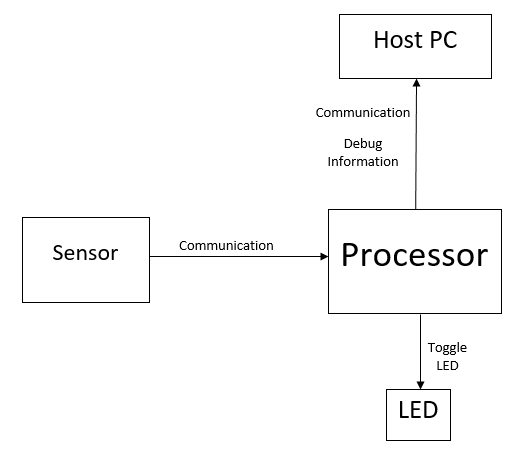
\includegraphics[scale=.8]{hardware-schematics-development.png}
	\caption{Hardware Block Diagram - Development}
	\label{fig:hardware_schematic_development}
\end{figure}

\begin{figure}
	\centering
	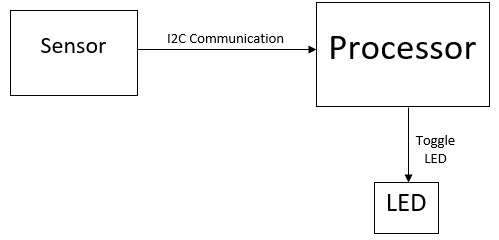
\includegraphics[scale=.8]{hardware-schematics-final.png}
	\caption{Hardware Block Diagram - Final}
	\label{fig:hardware_schematic_final}
\end{figure}
\namedsection{ARM Cortex M0 Processor}{Pasat}

\note{talk about limitations of the processor ie no hardware divide or floating point arithmetic}

This section discusses one of the main requirement and one of the essential aspects of our project, ARM’s Cortex M0 processor. This processor is a member of the Cortex-M family and offers a great tradeoff in terms of costs and performance/functionality. It has been designed in order to allow intelligent compromises in terms of power usage, computational power and in the simplicity of the design. It implements a simplified version of the Advanced Microcontroller Bus Architecture (AMBA), the AMBA-Lite bus which allows connection to different peripherals. In this way, the Cortex-M0 generally acts as the master device and the peripherals act as slaves. In figure \ref{fig:cortexm0ds}, the schematic for the processor can be seen.\\
\begin{figure}
\centering
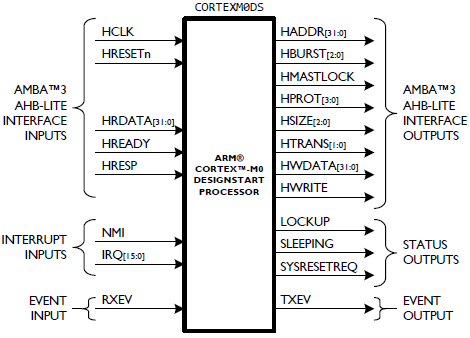
\includegraphics[scale=0.7]{figures/cortexm0ds_schematic.PNG}
\caption{Cortex M0DS schematic \label{fig:cortexm0ds}}
\end{figure}
\clearpage

\begin{figure}
\centering
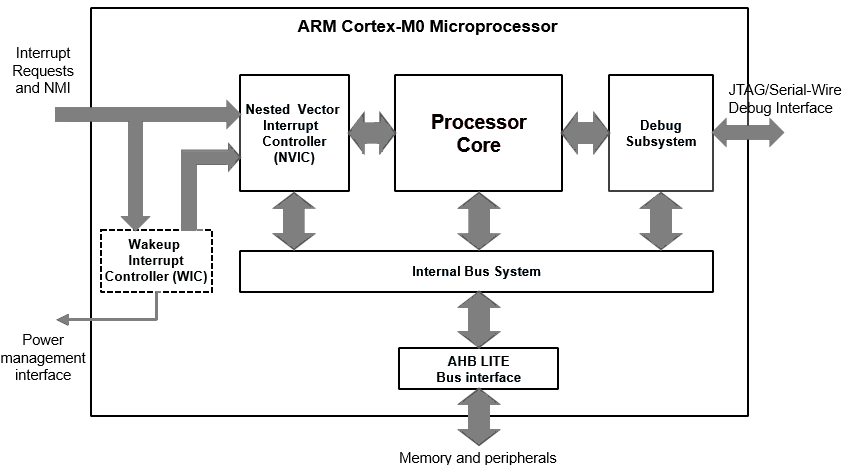
\includegraphics[scale=0.7]{figures/arm_cortexm0_microprocessor.PNG}
\caption{Cortex-M0 Block Diagram \label{fig:cortex_block}}
\end{figure}

The Cortex M0 has a 32-bit reduced instruction set computing(RISC) processor. It uses the ARMv6-M(Microcontroller), which is a subset of the ARMv7-M profile but it includes fewer instructions. The Cortex M0 is based on a Von-Neumann architecture, having both data and instructions share a single bus interface. It provides a Debug Extension that includes some architectural extensions to support debugging. The ARMv6-M offers support for 56 instructions as a subset of  Thumb-1(16-bit) and Thumb-2(16/32b-bit) which are present in the ARMv6T2. The Cortex M0 block diagram can be seen above in figure \ref{fig:cortex_block}. 

The Processor Core contains the internal registers, data path, ALU and control logics. The Cortex M0 has a three-stage pipeline: fetch, decode and exection and includes the 32-bit registers for general and special usages. The Cortex M0+ has only a two-stage pipeline to reduce the power usage.

The Nested Vectored Interrupt Controller(NVIC) handles up to 32 interrupts request signals and one NMI(Non-Maskable Interrupt). It also fulfils tasks such as comparing priorities between  interrupt requests and the current priority level. 

The Bus system contains the internal bus system, the data path in the processor core and the AHB LITE interface unit which is an on-chip bus protocol which enables some features required for high-performance, high clock frequency systems. 

The Debug system handles the program breakpoints, debugging control and the data watchpoints. This can put the processor in a  static state in order for the programmer to evaluate and analyse the status of the processor in that specific moment.

The Wakeup Interrupt Controller (WIC) is important for this project because it is used in low-power applications. The microcontroller can be set to enter sleep mode by turning off most of its components. If a interrupt request is sent, this component can inform the unit that handles the power management to power up the system.

Floating point is the formulaic representation for a real number for approximating it in order to obtain a balance between precision and range. Basically, it refers to the fact that a number's decimal point can "float", meaning  that is can be placed anywhere relative to significant digit from the number. One of the major challenges which were encountered in the use of the Cortex M0+ is the absence of floating point arithmetic on the device. This was mitigated by scaling each double value by $2^{12}$ and taking the integer part. After each multiplication, the value is bit-shifted by 12 to keep the scale factor consistent. This will be described late in more detail in section \ref{sec:floating-point}.

Real-time integer division supplied by ARM Libraries are faster then standard division routines for larger quotients, but slower for typical  quotients. Real time division is not available in the Cortex-M0+, so this was another issues that was overcome in our design. This was done by done by finding alternative methods to avoid division. More detail about this can also be found in \ref{sec:floating-point}.
\begin{figure}
\centering
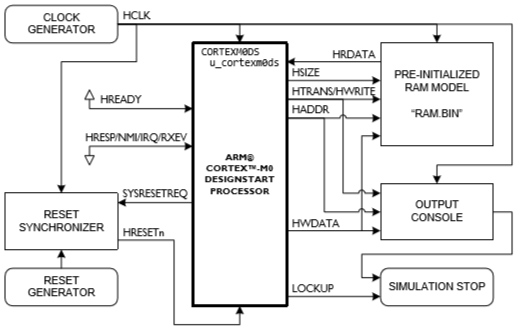
\includegraphics[scale=0.7]{figures/test_bench_schematic.PNG}
\caption{Cortex M0 test bench schematic} \label{fig:test_bench}
\end{figure}

\note {cite ARM DesignStart notes}
Through ARM, we managed to gain access to a fixed configuration of the Cortex-M0 Processor know as Cortex-M0 DesignStart. This simplified version offers us access to a Verilog version of the Cortex-M0 under the form of an obfuscated and preconfigured netlist, but it can be synthesized. This package offers us some Verilog codea test-bench which allow a simulation of the Cortex-M0 DesignStart module connected to a memory model and a clock and reset generator. It also include a basic C helloworld.c program. The schematic for the test-bench can be seen in figure \ref{fig:test_bench} and it connects the CORTEXM0DS to a memory model, a clock and a reset generators.

The tool used for simulating the test-bench is ModelSim, which is a tool that offers the possibility of simulating hardware description languages such as Verilog and VHDL. A new project must be created in ModelSim to which we add the Verilog files provided in the package, the test-bench and another binary file provided, ram.bin, which is an example memory image for the processor. The file is loaded at the beginning of the simulation by the test-bench.  The memory image is used for the helloworld.c program, which is used by the test-bench to write a message to the simulator's console and after that end the simulation. The result of the simulation can be seen in

Also, access was given to the CM0DS example design kit which contains various AHB-Lite peripherals and infrastructure components, useful to create complete systems. Before implementing the actual algorithm on the FPGA, a more basic simulation needs to be conducted on the platform to assure that it is compatible with the specific FPGA used. Next, the analysis of the sensors used for our project will be discussed. After that, discussions related to the about mBed platform which contains the Cortex M0+ and the Digilent Nexys4 FPGA board on which we aimed to implement the microprocessor as an extension will take place.

\section{Component Research}

\namedsection{FPGA}{Pasat}

\subsection{Introduction}

A FPGA (field-programmable gate array) is an semiconductor device which is has a matrix of CLBs (configurable logic blocks) connected through programmable interconnects. One main advantage of FPGAs is that the can be preprogrammed after they are manufactured in order to fit desired functionalities and requirements, such as the ones required by our team's project.
\\\\
The two devices we are using, the FPGA and the Microcontroller, are two very different devices. The microcontroller has the chip already designed. The programmer simply writes the software in C or C++, then it is compiled into a hex file that is loaded on the microcontroller. The program is stored in the flash memory until is is replaced or erased.
\\\\
FPGAs are different in this sense. The circuit is completely designed by the programmer. The processor must be created and can be as simple as an and gate or can be our Cortex M0+. HDL is used to write the design, which is then synthesized into a bit file which configures the FPGA. One small problem with this is the fact that it stores the configuration in the RAM, so once the power is gone, the configuration is lost.
\\\\\
The board used for this project is the Xilinx Digilent Nexys4, which can be seen in figure \ref{figure: nexys4} on the next page. It is based on the Artix-7 that has the lowest power consumption at 28nm and is optimized to give the design the highest performance. We chose this board because it is a large, high-capacity FPGA board that would be sufficient for our project. Another reason is the fact that is has several built in peripherals, such as accelerometer, which would be useful for the exercise detection. 
\begin{figure}
\centering
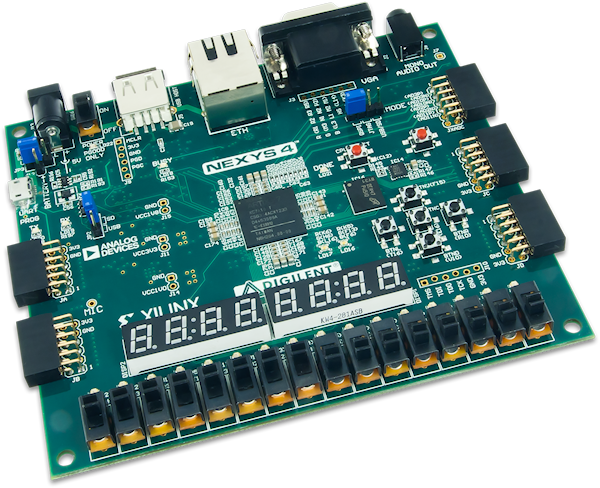
\includegraphics[scale=0.7]{figures/nexys4.PNG}
\caption{Xilinx Digilent Nexys4 \label{fig:nexys4}}
\end{figure}

Next,the implementation of the Cortex M0 DesignStart on the FPGA board will be discussed. The system will have a Cortex-M0\_DS processor, a preloaded memory with a program that fetches constants from a memory at regular intervals, a reset and a pattern detector attached to the bus so when a specific pattern appears on the data bus, the LED turns on and when another patters appears it will turn off. The Cortex-M0\_DS  includes only the processor a non-synthesizable testbench. Other parts will need to be implemented in order to create an synthesizable system: a software executable image, a memory holding the program, a system clock, a detector module for the command LED and a reset synchronizer. This section will be divided into: software development and simulation, system implementation and functional simulation. All of these sections will be discussed in detail in what follows.

\subsection{Software development and simulation}
In this section, a software program that will verify the memory fetches of some predefined constants. The program used for this will be ARM Keil μVision, which is a IDE(Integrated Development Environment) which allows quick and easy building of projects and includes other facilities such as: make facilities, source code debug, program debug and complete simulations.

To start, a new project must be created in μVision. Next, the device must be selected device database so ARM-ARM Cortex M0 plus-ARMCM0P is selected which can be seen in figure \ref{armcm0p}.
\begin{figure}
\centering
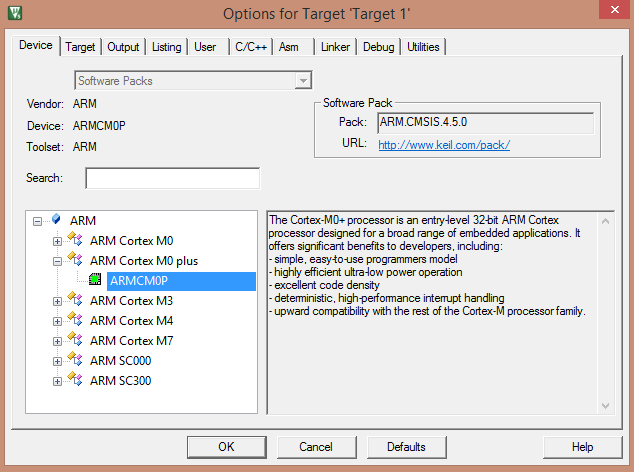
\includegraphics[scale=0.7]{figures/armcm0p.PNG}
\caption{Selection of the Cortex M0+ for the μVision project} 
\label{fig:armcm0p}
\end{figure}

After this is selected, the options menu is accessed for this device. Next, the target options need to be accessed and the following modification need to be made:

- under Target section, the Read/Write Memory Areas, RAM1 starts at 0x0 and has the size of 0x400000 (this setting is used to create a linker scatter file. Another requirement for this is the having the Use Memory Layout from Target Dialog enabled in the Linker section);

- under Output section, the Debug Information and Browse Information sections need to be ticked(this defines the resulting output files from the tool chain and allows the user programs to be started after the building process is complete);

- under Listing section, all the default selected features stay the same(here all the listing files generated by the tool chain are specified);

- under User section, in Run\#1:"fromelf -cvf code.axf --vhx --32x1 -o code.hex" and Run\#2:"fromelf -cvf code.axf -o disasm.txt" in Run User Programs After Build/Rebuild those code lines are inserted in order to create a .axf file from the .hex file;

- under C/C++ section, the One ELF Section per Function is unticked and the Warnings are set to <unspecified> (here C/C++ specific tool options are set);

-under Asm section, all the settings are kept to default also( this allows the setting of specific Assembler tool options);

-under Linker section, the R/W Base entry is deleted and only the R/O Base: 0x00000000 remains(linker settings are required in order to configure the physical memory location of the target). The location of memory classes and sections is defined here.

-under Debug section, the default settings for µVision4 Debugger stay the same;

-under Utilities, the Use Target Driver for Flash Programming in the Configure Flash Menu Command is left checked.

After all of these steps have been done,it is now time to add assembly file provided by ARM, the cm0dasm.s to the source. Taking a look at the reset handler, which can be seen in \ref{reset_handler},  the value 0x55 is written to the LED when a specific pattern is detected and 0xAA if another pattern is detected.
\begin{figure}
\centering
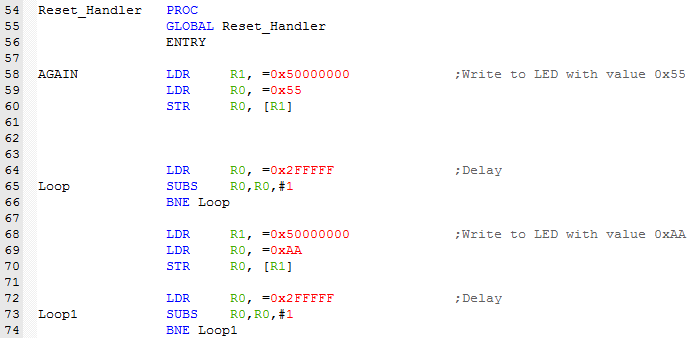
\includegraphics[scale=0.7]{figures/reset_handler.PNG}
\caption{Reset handler} 
\label{fig:armcm0p}
\end{figure}

After the successful building of the code.hex should be created and converted into a .axf because it was set in the User section. The .axf file needs to be converted to a .bin in order to program the FPGA. The MDK/Keil offers a tool called "fromelf" which can do this conversion. It is called in the following way:

fromelf --bin --o code.bin code.axf

This can be ued to program the FPGA. Now, the implementation of the Cortex-M0+ will be discussed.

\subsection{System Implementation}

ARM offers access to packs that makes the implementation of the Cortex M0+ on the FPGA is discussed. The components which will be used are: the ARM Cortex-M0 processor, the AHB-Lite system bus and two AHB peripherals: the program memory(which will be implemented using on-chip memory blocks) and a simple LED peripheral.

The software used for this implementation is Vivado Design Suite. This software is produced by Xilinx and is used for synthesis and analysis of HDL designs and is a improved version of the Xilinx ISE which also allows features such as system on a chip development and a high-level synthesis. A new project must be created

The ARM DesignStart  package which contains the logic of the ARM Cortex-M0 processor written in Verilog and can be synthesized and implemented on a FPGA platform. The Cortex-M0 DesignStart will be used, which is a simplified version of the industry Cortex-M0 processor, but has some features reduced which are not essential for this project such as in the number of interrupts(from 32 to 16). Two verilog files are included in this pack:  cortexm0ds\_logic.v and CORTEM0DS.v. The cortexm0ds\_logic.v contains the Cortex-M0 DesignStart processor logic level Verilog file, while the CORTEXM0DS.v includes the Cortex-M0 DesignStart processor macro cell level.

The software code needs to be compiled to machine code in order to program the processor.
\namedsection{mBed}{Gupta}

\note{Add a plan?}

\subsection{Introduction}

mBed is a platform which implements ARM 32-bit processors within micro-controllers which is primarily developed by ARM. They are of the DIP form factor with 40 pins. It features an online SDK allowing for the development of projects online. It permits code to be written online as well as compiled into a binary compatible with the board being used. This binary can then be downloaded removing the pre-requisite of having the ARM toolchain available locally. The manner of uploading to the mBed is relatively straight forward with the presence of the mBed interface. \cite{mbed_website}\todo{Try expanding on this section}

This interface exposes a Mass Storage device to the host computer via a USB connection allowing for binaries to be uploaded in a drag and drop manner. The interface is also connected with the target chip using a JTAG connection allowing for it to program its flash memory. When the reset button is pressed, the interface checks the storage for the newest binary file and, should it not be programmed within the device already, will program the binary provided into the flash memory of the chip. \cite{mbed_website}\todo{Try expanding this section as well}

\subsection{Why the mBed}
\note{Need a better name for this subsection?}
\note{Talk about the availability of other required protocols}

When initially looking at various ways to emulate the sub-threshold version of the ARM Cortex M0, using an existing non sub-threshold version of the ARM Cortex M0 was considered. This involved searching for some form of micro-controller or device which would allow for programming of the processor. This lead to the mBed family which appeared easy to program and use featuring ARM processors. Within the mBed family of micro-controllers, the LPC11U24 model uses an ARM Cortex M0 as its processor.

The requirements for this project require the processor to be emulate the sub-threshold version which operates with a system clock in the range of a few hundred kHz to a few MHz. This would require a clock in the micro-controller which can operate at these frequencies and also be able to be set as the system clock.

The device typically runs at 48MHz using its Internal RC oscillator (IRC) as its system clock. However, it also has the ability to switch its system clock to be sourced from the internal Watchdog oscillator instead. 

This oscillator consists of two parts, an oscillator function which generates an analog clock (\verb|Fclkana|) as well as a divisor (\verb|DIVSEL|) which is used to divide the analog clock to the required output frequency (\verb|wdt_osc_clk|). The output frequency can be calculated using Equation~\ref{eq:wdt_osc_clk} and is within the range $ 9.4 $ kHz $ \leq \verb|wdt_osc_clk| \leq 2.3 $ MHz. \cite{mbed_datasheet}

\begin{equation}
	\label{eq:wdt_osc_clk}
	\verb|wdt_osc_clk| = \frac{Fclkana}{2 * (1 + DIVSEL)}
\end{equation}

Some concerns were made realising that the Watchdog oscillator has an error margin of $\pm 40\%$ for the frequency of Fclkana. In a meeting with the client, it was decided to carry forward with the device while paying attention to this margin and analysing the impact of it upon the project.

\subsection{I2C Communication}

\subsubsection{Sensor library}

The sensor used in this project, the MPU6050 within a Xadow board, has an online library available \cite{sensory_library}. It contains two separate classes, one called I2Cdev and the other MPU6050. 

The I2Cdev class contains an interface to the processors I2C class expanding its functionality and allowing for more abstract functions for the MPU6050 class. For example, functionality for reading or writing multiple bytes or words were implemented within this class.

The MPU6050 class contains the functionality for configuring the sensor itself as well as reading data that it collects. It uses the I2Cdev class for communicating with the sensor.

The libraries are written for use with the Atmel chipset which use different libraries than those used by the ARM chipset. This poses a small issue as this means that the I2Cdev class would be incompatible for the ARM chip in use. In turn, due to the reliance on this class by the MPU6050 class, it would also be incompatible. 

This can easily be rectified by re-writing the I2Cdev class to make it compatible with the ARM libraries, which would also make the MPU6050 compatible.

\note{Talk more about this - i2c\_start, i2c\_stop}

\subsection{Watchdog Oscillator}

As mentioned before, one of the objectives of this project is to operate at a low operating frequency. It has already been seen that the Watchdog oscillator can operate in the desired frequency range using an analog clock as well as a divisor. 

To configure the Watchdog oscillator, it needs to be configured, powered on and then switched to. To do this, there are three registers that need interaction with to complete. The first register is the Watchdog oscillator control register (\verb|WDTOSCCTRL|) which contains the \verb|DIVSEL| and \verb|FREQSEL| talked about earlier. 

The lowest five bits of the register contains the unsigned value of \verb|DIVSEL|, hence allowing it to be within the range $ 0 \leq $ \verb|DIVSEL| $ \leq 31$. Thus, allowing for the divisor being within the range $ 2 \leq $ divisor $ \leq 64$.

The next four bits contains a value for \verb|FREQSEL|, where a value within the register corresponds to a different frequency with the relationship that can be seen in Table~\ref{tab:freqsel}.

\begin{table}
	\centering
	\begin{tabular}{|c|r|}
		\hline
		Value & Frequency \\
		\hline
		0x1 & 0.6 MHz \\
		0x2 & 1.05 MHz \\
		0x3 & 1.4 MHz \\
		0x4 & 1.75 MHz \\
		0x5 & 2.1 MHz \\
		0x6 & 2.4 MHz \\
		0x7 & 2.7 MHz \\
		0x8 & 2.0 MHz \\
		0x9 & 3.25 MHz \\
		0xA & 3.5 MHz \\
		0xB & 3.75 MHz \\
		0xC & 4.0 MHz \\
		0xD & 4.2 MHz \\
		0xE & 4.4 MHz \\
		0xF & 4.6 MHz \\
		\hline
	\end{tabular}
	\caption{FREQSEL table for WDTOSCCTRL register}
	\label{tab:freqsel}
\end{table}

With the available frequency values and divisors, it confirms the range that the Watchdog oscillator achieves which was given earlier.

\subsubsection{Analysing the error margin}

It is known that the Watchdog oscillator has an error margin of $ \pm 40\%$, the actual impact this would have however is unknown. According to the data sheet \cite{mbed_not_datasheet}, the primary reason for this is temperature. Due to the conditions that the device is intended for, upon a plane, the ambient temperature can be assumed to not be at extreme temperatures in either direction, hence should not be an issue. There was a hypothesis that the power supply voltage could also affect the frequency of the oscillator. 

To test this, the supply voltage for the mBed is varied and the output frequency of the oscillator is checked. There was an issue due to the fact that the mBed does not provide a breakout pin for the CLKOUT pin. To get around this, the while loop is programmed to contain only toggling a pin. The act of toggling the pin should take a constant number of cycles each time, hence the frequency of that pin should be proportional to the frequency of the clock. Hence, can be used to measure deviations in the system clock.

Implementing this with the watchdog oscillator using a FCLKANA of 0x1 (0.6 MHz) and a DIVSEL of 2 (Divisor of 6), the Watchdog oscillator oscillates at 100 kHz. Measuring the frequency of the pin over a range of voltages shows no change in frequency, hence disproving the hypothesis that the voltage would also affect the operating frequency.

\subsection{Serial Communication}

For the purposes of debugging, serial communication was used to extract information from the device and onto the host computer. To accomplish this, a C232HM cable \cite{c232hm_datasheet} was used to interface with the host computer, via USB, and the mBed, via Serial pins 9 and 10. The baud rate was left at the default value of 9600 and to test the communication, the mBed was programmed to send "Hello World!" to the host pc via Serial communication.

This communication was done when the device was operating at its default frequency of 48 Mhz where the libraries have the correct default values set in the registers to enable the correct divisors to enable the device to operate at 9600 baud. However, these would not be viable values when using the Watchdog Oscillator as the system clock.

\subsubsection{Serial Divisor}

To enable the device to communicate with the desired baud rate when the system clock is set at a lower frequency, the divisor needs to be configured. There are multiple registers that need to be modified to achieve this. The first two are the DLL and DLM registers. These registers, within the lowest eight bits, contain the DLL and DLM bytes respectively, where DLL is the least significant byte of the Divisor Latch (DL) and DLM is the most significant byte.

For access to be granted to the DL, the Divisor Latch Access Bit (DLAB) needs to be set. This value is stored within the Line Control Register as the seventh bit. The final register is the Fractional Divide Register which contains the DIVADDVAL and MULVAL values. DIVADDVAL is stored within the lowest four bits, whilst MULVAL is stored within the next four lowest bits. 

Using these values, the baud rate can be calculated using Equation~\ref{eq:serial_baud_rate} where PCLK is the clock frequency\cite{mbed_datasheet}.

\begin{equation}
	\label{eq:serial_baud_rate}
	UART_{baud rate} = \frac{PCLK}{16 * (256 * DLM + DLL) * (1 + \frac{DivAddVal}{MulVal})}
\end{equation}

Within the mBed datasheet \cite{mbed_datasheet}, a methodology for calculating these values is provided which can be seen in Figure~\ref{fig:serial_algo}. Along with the algorithm, a look up table is provided which can be used to translate a FR value to DIVADDVAL and MULVAL values. 

\begin{figure}
	\centering
	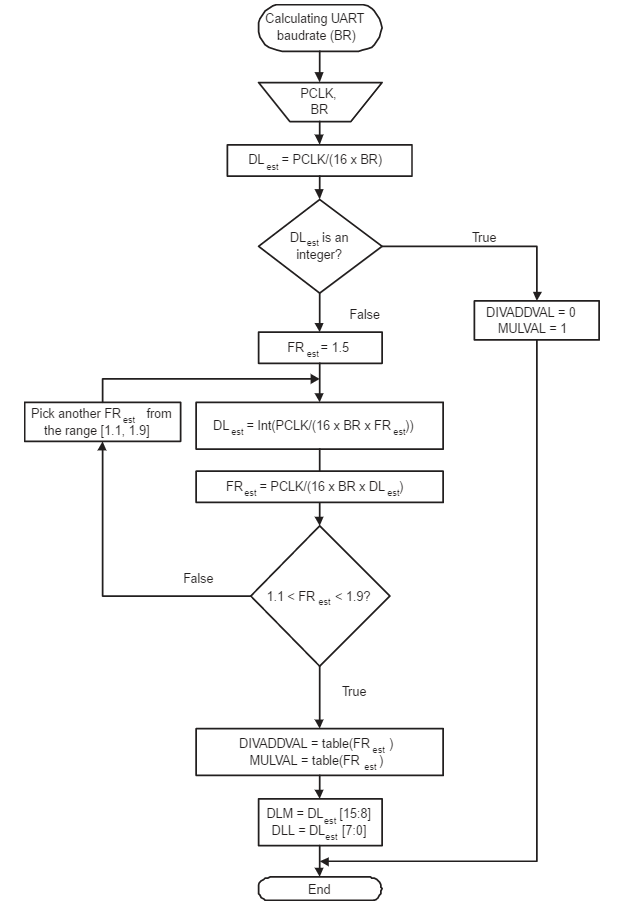
\includegraphics[scale=.85]{usart_algorithm.png}
	\caption{Algorithm to calculate required values for Serial baud rate}
	\label{fig:serial_algo}
\end{figure}

\subsubsection{Auto-Baud}

Another option to account for this is a feature provided within the processor called Auto-Baud\cite{mbed_datasheet}. This is where the device waits on receiving communication upon its RX pin and of the data coming in, it measures the baud rate between a falling edge and a subsequent rising or falling edge depending on the mode set within the registers.

Using this information, the required registers are set to enable Serial communication such that the device can communicate at the required baud rate. To enable an effective method for enabling auto baud, a python script was created which can be used on the host PC. This script continuously sends the character 'g' whilst also receiving and printing bytes. The continuous stream of 'g's gives a signal for auto baud to configure itself and should the device be reset during communication it will be configured automatically after reset should the script be running.

\subsection{Getting Sensor Data}

With the sensor libraries re-written to be compatible with the ARM libraries, the sensor can be interfaced with the mBed. Upon the sensor, all pins used were on Junction 4. This pins connected between the mBed and sensor were the data line, pins 28 and 3 respectively, as well as the clock line, pins 27 and 2 respectively. These pins were also connected to pull-up resistors with values of 2.2k\ohm. Power was also supplied to the sensor from the mBed from its 3.3V Regulated Output which went to pin 1 of the sensor along with a common ground between the Ground pin of the mBed and pin 6 of the sensor. 

Once done, it was possible to extract sensor readings from the device, depending on what data is required a variety of different functions from the library can be used.

\begin{description}
	\item[Accelerometer X axis] \hfill \\ getAccelerationX
	\item[Accelorometer Y axis] \hfill \\ getAccelerationY
	\item[Accelorometer Z axis] \hfill \\ getAccelerationZ
	\item[Accelerometer all axis] \hfill \\ getAcceleration
	\item[Gyroscope X axis] \hfill \\ getRotationX
	\item[Gyroscope Y axis] \hfill \\ getRotationY
	\item[Gyroscope Z axis] \hfill \\ getRotationZ
	\item[Gyroscope all axis] \hfill \\ getRotation
	\item[Accelerometer and Gryoscope all axis] \hfill \\ getMotion6
\end{description}

\todo{Do something about this}

Thus allowing for a variety of possibilities for obtaining data from the sensor, as should only certain data be required, a function can be chosen which reduces the amount of data being received, hence reducing the communication time between the mBed and sensor.

\subsection{Getting the desired sampling rate}

The model employed requires a set sampling rate, and to minimise the communication between the mBed and device to minimise processing, the mBed should sample the sensor at the sampling rate required by the model. To achieve this, there a few different parameters tweaked, specifically the Watchdog \verb|FCLKANA| and \verb|DIVSEL| as well as SCLL and SCLH for the I2C clock. These values represent the number of clock cycles the I2C clock remain low and high respectively, where the lowest value they may have is four. Thus, can be used to speed up or slow down I2C communication. \cite{mbed_datasheet} This can be summed in Equation~\ref{eqn:i2c_clock}.

\begin{equation}
	I2C_{clock} = \frac{CLK}{SCLH + SCLL}
	\label{eqn:i2c_clock}
\end{equation}

It was decided that the duty cycle of the I2C clock is 50\%, hence the value of SCLL and SCLH should be the same. A similar method, from when measuring the frequency of the oscillator with varying voltage via a pin, was used where the frequency of the pin is half the sampling rate. This because in one cycle of the pin, it goes through the while loop twice and the sensor is queried once each loop.

\subsection{Measuring power}

It is required to measure the power of the system as a requirement is for it to be low powered as the sub threshold processor will be operating at a low power. It was deemed unnecessary to measure the power consumption of the mBed because of the various peripherals which are also powered which would not be there on the sub threshold version as well as the fact that this processor is not designed for sub threshold power and the method ARM implement to achieve this may leave a different power fingerprint than the Cortex M0. 

The sensor however does not fall under the same conditions and thus, was analysed for its power usage. To do this a 100\ohm ~resistor was placed in series between the sensor and $V_{cc}$. Thus current would have to flow through the resistor to reach the sensor, allowing to measure the current by measuring the voltage across the resistor along with the relationship V=IR.

The power consumption of the sensor is not constant over time due to the fact that the sensor alternates between sleep mode and being awake. It also will consume more power when communicating over I2C as opposed to not. To account for this, the current and voltage is measured over time which is then averaged thus, giving the average power consumed by the sensor.

\begin{table}
	\centering
	\begin{tabular}{|l|r|r|}
		\hline
		Parameter & Mean Value & Standard Deviation \\
		\hline
		Resistor Voltage (V) & 0.0262 & 0.00198 \\
		Sensor Voltage (V) & 3.29 & 0.00133 \\
		Current (A) & 0.000262 & \\
		Power (W) & 0.00086198 & \\
		\hline
	\end{tabular}
	\caption{Power statistics for the sensor}
	\label{tab:power}
\end{table}

As can be seen from Table~\ref{tab:power}, the sensor on average took $861\mu W$ which can be considered low power. However, there is the potential for a lower power consumption, within the configuration used, the current flowing through the sensor was $262\mu A$, but the data sheet for the sensor says for the sampling rate and configuration that is being used, the typical value is $70\mu A$. This decrease would reduce the power consumption by over a factor of 3 leaving a power usage of $230\mu W$.

\subsection{Prototyping}

During development, breadboard was used to prototype the system with both the mBed and sensor placed upon. The power rails on the breadboard received power from the mBed which in turn received power from the host PC via USB. These conditions were acceptable when developing, however was impractical for moving the device to the foot for further testing. 

It was decided to create a small board for this purpose using veroboard which would be powered with a few AA batteries. This is beneficial as the board can be made to a desired size with on-board power alleviating the requirement of having a cable trailing to a computer as well as being more comfortable on the foot over the breadboard.

A design was created using fritzing \cite{fritzing} which can be seen in Figure~\ref{fig:veroboard_schematic}. The mBed has a $V_{in}$ pin upon pin 2 which can take from 4.5V up to 9V which is supplied using four AA batteries within two AA battery holders. To prevent the mBed from constantly being powered, a jumper is added to control whether the mBed receives power or not enabling for the device to be switched on or off at will. Power to the sensor is provided via the 3.3V regulated output of the mBed, which also is used by the pull-up resistors to hold the I2C lines high when not in use. Extra space was added above and below the sensor due to the fact that the physical board is larger than that in the CAD software upon that axis, thus requires more space to avoid colliding with the mBed or hanging off the edge of board.

\begin{figure}
	\centering
	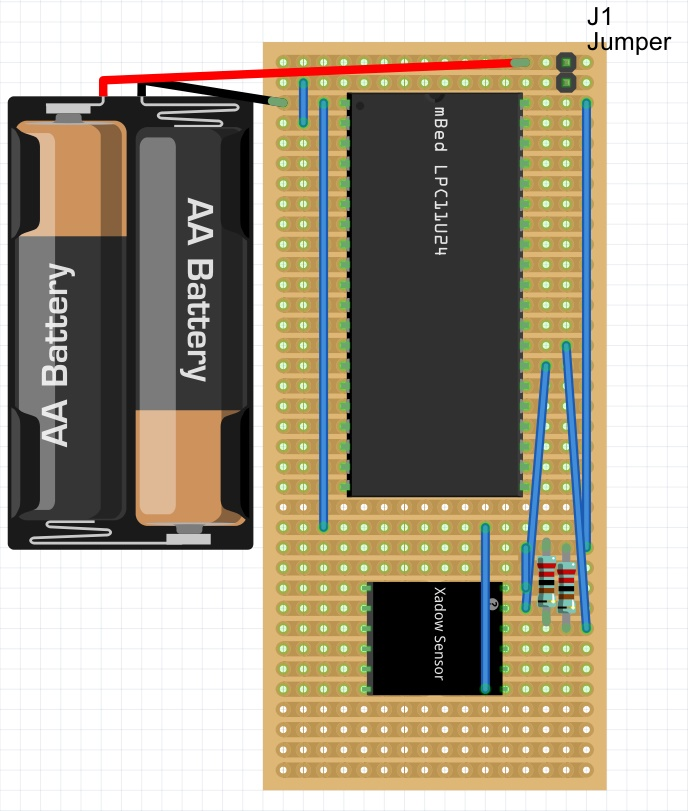
\includegraphics[scale=.6]{veroboard_schematic.png}
	\caption{Schematic for veroboard}
	\label{fig:veroboard_schematic}
\end{figure}

This was then built, as can be seen from Figure~\ref{fig:board}. To avoid having to solder on the actual mBed and sensor to the veroboard, female header pins are used in a manner similar to IC holders allowing for them to be placed and removed from the board as required. For compactness, the battery packs were attached to the underside of the board using velcro. 

\note{Limitations of mBed, e.g. hardware divide, floating point arithmetic}
\note{Configuring Watchdog Oscillator for main clock}
\note{SPI mBed library cannot be compiled because it is bigger than the flash memory}
\note{Bitshifting gives random outputs fun -- little endian}
\namedsection{Sensor}{Gupta}

The sensor chosen, Xadow IMU 6DOF which uses the MPU6050 chip, allowed for a great deal of versatility by means of configuring the various registers contained within the MPU6050. This allowed for the option to use what was required by the sensor and nothing else, thus helping to minimise the power consumption of the device where possible. \cite{sensor_specs}

The primary usage of the sensor to the project, are the 3-axis accelerometer and gyroscope which can be used to measure the acceleration and angular velocity upon the foot. The data collected can be extracted from the sensor using I2C communication. 

When reading values from the sensor, the raw value is received. This is a value in the range -32768 to 32767 which then needs to be translated to an actual value. The relationship between the raw value and the actual value is dependant on the sensitivity configured for the accelerometer or gyroscope. The typical values for the sensitivity are $\pm 2g$ and $\pm 250~\degree / sec$ respectively. The sensitivity can be considered the maximum value that the sensor will provide, ie the sensitivity values are also the values at either end of the raw value range. This leaves a linear scale in between allowing for easy calculation of the reading given the sensitivity and the raw value. For example, a range of $\pm 2g$ and a raw value of -32768, -16384 and 0 would give actual values of -2, -1 and 0 respectively. Thus, it can be inferred that the greater the sensitivity, the lower the resolution available. \cite{sensor_raw_explanation}

\subsection{Gyroscope}

The gyroscope can operate at a variety of sensitivities, from $\pm 250$ to $\pm 2000~\degree / sec$ and while active draws $3.6mA$. The sensitivity can be configured within Register 27 (Gyroscope Configuration). Bits 4 and 3 contains a value telling the sensor what sensitivity to use, these values and corresponding sensitivities can be seen in Table~\ref{tab:gyro:range}. \cite{sensor_registers}

\begin{table}
	\centering
	\begin{tabular}{|c|c|}
		\hline
		Value & Sensitivity \\
		\hline
		0 & $\pm 250~\degree / sec$ \\
		1 & $\pm 500~\degree / sec$ \\
		2 & $\pm 1000~\degree / sec$ \\
		3 & $\pm 2000~\degree / sec$ \\
		\hline
	\end{tabular}
	\caption{Values to select gyroscope sensitivity}
	\label{tab:gyro:range}
\end{table}

\subsection{Accelerometer}

The sensitivities that the accelerometer can operate at range between $\pm 2$ to $\pm 16g$ and typically under normal operation draws $500\mu A$. The sensitivity can be configured within Register 28 (Accelerometer configuration) in bits 4 and 3. Possible values within these two bits as well as corresponding sensitivities can be seen in Table~\ref{tab:accel:range}. \cite{sensor_registers}

\begin{table}
	\centering
	\begin{tabular}{|c|c|}
		\hline
		Value & Sensitivity \\
		\hline
		0 & $\pm 2g$ \\
		1 & $\pm 4g$ \\
		2 & $\pm 8g$ \\
		3 & $\pm 16g$ \\
		\hline
	\end{tabular}
	\caption{Values to select accelerometer sensitivity}
	\label{tab:accel:range}
\end{table}

The sensor also supports a low power accelerometer which uses only the accelerometer at a configured frequency. This takes less current than typical usage, however is dependant on the sampling frequency of the accelerometer. This is done by putting the device into a cyclic sleep mode where it wakes up at the wake frequency to take a single set of readings from the accelerometer before going back to sleep.



	% User study chapter
	\chapter{User Study}
As seen from the software section, it was decided that a machine learning approach would be most appropriate for developing the algorithm to detect exercises. In particular, a Multilayer Perceptron was the chosen type of machine learning algorithm. 

Apart from performing the actual optimisations on the algorithm, another important step was to gather training data which could be used to generate a model for the algorithm to use. The model plays a vital role because it is used to make classifications of new data based on the data it has been trained on.

The data which is involved are the readings from sensors which are attached to the body of a person when they are performing the exercises. As it is the intention for the system to be used by many different people who travel in planes, it was decided to gather the training data using a user study. This is because each individual has slight variations in the way they perform exercises so in order to improve the robustness of the system we collected movement data from 20 different people. This movement data could then be combined as the training data to form a model capable of correctly classifying exercises for most people.

\section{Study Preparation}
Before performing studies involving participants who are not actually members of the project it is required to gain ethical approval. This is a requirement put in place from the University of Southampton and also covers the legal requirement of data protection when dealing with participant’s personal data. Faculty ethics committees review applications for ethical approval and once they are approved insurance and legal cover is provided. Therefore, it is highly important to follow the approval process as it helps to make sure there is enough detail and planning in the study to help keep participants safe.

To get advice with the application process, contact was made with the University of Southampton Safety and Occupational Health department <ref>. In a meeting between the groups user study lead and members of SOH it was decided that the study should take place in a private room where there would not be any interruptions and assistance was provided with booking a lab room in the Phycology department for this purpose. Further assistance was also given for finding the contact details of first aiders.

\section{Ethical Approval Process}
Throughout the application process, heavy reference was made to the instructions and guideline documents provided by the Ethics and Research Governance Online website <ref>. One of the key things that are used to classify studies are study characteristics which are a list of areas where potential risks could be introduced ranging from low to high likelihood. As our study involved wearable technology, this counted as being intrusive which in turn meant there was a risk of harm and these are two medium risk study characteristics.

This meant that the user study had to provide consent forms so that participants could provide their consent for taking part in writing. However, this also meant that personal data was collected in the study which caused another study characteristic to be matched.

Overall, this required several documents to be submitted as part of the ethics application. These included the consent form as already mentioned and participant information which clearly stated to the participants what will be required of them in the study. On top of this, a data protection act plan which outlined how participant’s personal data will be kept safe was also submitted along with a risk management plan which had to identify possible ways a participant might get injured and how these risks would be reduced. A debrief plan which stated how participants could be told of the results of the study was also included as were contact information and technical details documents to provide even further details about the study.

In this project, there were two areas where user studies could have been required. One was to collect movement data to train the algorithm by generating a model as already mentioned. The other area was to perform a user study to test the final system and measure its accuracy. As applying for ethics approval is a very time consuming process, it was decided to incorporate both areas into a single study. This was possible because both areas involve the participants performing exactly the same actions, it was only what was being recorded that changed. This was made clear throughout the ethics application which eventually led to it being approved.

\section{During the Study}
In the end, only the first area of the user study was performed for collecting movement data to train the algorithm. Specifically, accelerometer and gyroscope sensor data was required to be collected so that the effectiveness of the two at training the algorithm and accurately classifying exercises could be compared.

At this stage in the project, the prototype device was not yet ready to be used to record the movement data so a mobile phone with inbuilt accelerometer and gyroscope sensor was used instead. The Physics Toolbox Suite Version 1.4.4 app <ref> was used to record data directly from the phones sensors by allowing us to choose which sensors to use.

For each participant, the phone was strapped to various parts of their body using Velcro. These positions included the top of the right foot, and the outer side of their upper right arm. It was also made sure that these positions and the orientation of the phone were the same for each participant in order to make sure the data was consistent. This was vital as the data from each participant was combined to form the overall training data.

When the phone was attached to the foot, each participant was sat down and performed the foot rotation exercises where they stretched out their legs and slowly rotated their feet in both clockwise and anticlockwise directions about 10 times each. Also while sitting down, each participant performed the ballerina exercise where they placed their feet on the ground and raised their heels, followed by raising their toes and rolling back their heels to the ground. This was also repeated about 10 times. Walking movement data was also collected while the phone was on the foot. The purpose of collecting this was to use it to train the algorithm to not classify walking as exercise.

When the phone was attached to the arm, the participants were told to do the shoulder rolling exercise where the shoulders were rolled forwards approximately 10 times.

Each of these exercises was repeated twice. One time for the accelerometer data and one for the gyroscope data. At the end of each exercise, the results were emailed to a member of the group who made them available on a Git repository.

\section{Classification of Results}

	% Project management chapter
	\chapter{Project Management}


	% Results chapter
	\chapter{Results}

We have seen the methods that were used to research and train a neural network capable of recognising exercise, and then the work to implement this into a program capable of running on a Cortex-M0, which was developed to act as a emulation platform for the proposed sub threshold device. This chapter evaluates the outcomes of this work, highlighting the successes that have been made, and analysing where further development may be required.

\namedsection{Algorithm Accuracy \label{sec:alg-accuracy}}{Shepherd}

As discussed above, the team was not able to complete a second user study on the device, which means a detailed analysis of the accuracy of the algorithm may not be possible. Instead, the group have used their own members to experiment with the device; although this sample size is smaller than ideal, and as such any results may not be particularly statistically significant, the group felt this would provide a suitable proof of concept, and a good data point on which to base future work.

The team's early tests showed that the device is able to correctly identify a movement as exercise when the device was rotated in speed and fashion in accordance with the specifications. However, some team members found the device harder to use than others, suggesting that it may be too well trained to the `perfect' form of exercise. Should the device be developed further, it may aid its usability to address this drawback.

It also appears that the device's accuracy is affected by its angle on the foot to a far higher degree than the team were expecting - as such, when held flat and the exercises are performed in the hand, the accuracy is much higher than when it is attached to the foot. The angle is, perhaps, a factor which should be given greater weight when training models in the future.

We have found that the device's ability to ignore false positives is reassuringly high; to test this, members wore the sensor both during `random' foot movements, and during walking, neither yielding sustained exercise classifications. When exercise was detected incorrectly, this tended to be for short instants, making the likelihood of confusing an end user very low. The short time associated with mis classifications could also be used as a factor for more advanced heuristics to be added in the future, rather than requiring substantial amendments to the underlying classification code or model.

\namedsection{Size Analysis}{Shepherd}

In order to assess the overall size requirement of the completed algorithm, two areas of interest were identified: The Binary Size, which specifies the FLASH memory requirement, and the total size of code and in-program memory, which specifies the amount of RAM required. These items can be further split into three areas of investigation: The Code Size, The Heap Size and the Stack Size.

\subsection{Binary Size}

Finding the overall size of the binary file is a trivial task, simply running \verb|du -b output.bin| on a Linux-like console gives the result of 3168 bytes, or 3.09kB. However, it is important to assess the contributing factors to this size. The sections which are included in the compiled binary are \verb|.text|, which contains the program code and constant values, \verb|.data|, non-zero initialisations for the heap and finally, \verb|.ARM.exidx| which is an 8 byte section required for stack unwinding.

The size of \verb|.data| can be obtained by using arm's \verb|arm-none-eabi-size| command, which mirrors the functionality of GCC's \verb|size|; this gives a size of 108 for non zero heap initialisations. The majority of this is LibC values, with the exception of 4 bytes for an array index initialised to -1 which is used by multiple functions in the algorithm.

Finally, the size of \verb|.data|, which is now plainly 3052 bytes, must be assessed; again it is more meaningful to look into this in further detail. Fortunately, this can be performed by viewing the annotated disassembly of the binary. Table \ref{tab:prog-size} shows the breakdown of the binary file, with the values discussed in this section and the code split into logical areas.

\begin{table}[h]
    \centering
    \begin{tabular}{|l|c|}
        \hline
        Section & Size (Bytes) \\
        \hline
        System Interrupt Handlers & 204 \\
        System Init and Shutdown Code & 1184 \\
        Code & 1128 \\
        Constant Weights & 524 \\
        LibC Values & 12 \\
        .ARM.exidx & 8 \\
        Non-Zero Variable Initialisations for the Heap & 108 \\
        \hline
    \end{tabular}
    \caption{Binary File Size \label{tab:prog-size}}
\end{table}

\subsection{Memory Size}

A more important metric of size to quantify is the memory usage. At startup, the total binary is loaded into RAM. As discussed above, non-zero heap initialisations make up 108 bytes. However, during the system initialisation phase, a further 168 bytes are loaded onto the heap. After this, the heap does not grow any further, remaining at 276 bytes. As such, support for on-the-fly heap assignments (\verb|_sbrk()|) was removed from the mBed library to save space within the binary.

The final section of memory is the stack, which is perhaps the hardest area to accurately assess. For this, the compiler was passed the \verb|-fstack-usage| flag which prompts it to output the stack usage of each function; all of the algorithms had been designed to have static stack usage, which means the size of the stack is constant and therefore predictable, and the space is reserved at the beginning of the function. This was confirmed by inspecting the disassembly, in which the start of functions could be observed to contain a push instruction, followed by an amendment to the stack pointer to reserve the required space.

The stack usage of each function alone is not enough to assure the stack usage overall; this is because some functions call others, which means their stack values must be added. As such, a graph of each function and its stack usage was created, shown in figure \ref{fig:stack-calls}, with the calls between these added as vertices. The algorithm was designed to avoid any forms of recursion, so this graph does not contain any cyclic references which makes the task of determining the maximum stack usage more trivial.

\begin{figure}[!h]
    \centering
    \includegraphics{figures/stack-calls.pdf}
    \caption{Graph of Function Calls}
    \label{fig:stack-calls}
\end{figure}

\begin{figure}[!h]
    \centering
    \includegraphics{figures/stack-routes.pdf}
    \caption{Routes through Function Call Graph}
    \label{fig:stack-routes}
\end{figure}

We must first determine each of the possible stack states and their respective sizes, to do this we walk forward from main along each edge, adding the stack size of each node we encounter, until we can move no further. We then repeat this until no further routes can be found. Finally, the route with the maximum stack size is picked; this is the biggest the stack can ever be. This is shown by figure \ref{fig:stack-routes}, and from it is therefore clear that the stack never exceeds 120 bytes.

\subsubsection{Conclusion}

The total required RAM size can be calculated by the summation of the total binary size, the size of zero-initialised heap variables and the maximum stack size. This comes to 3456 bytes leaving 4736 bytes, or just over 4.6kB, free if deployed on an 8kB device. This space gives scope for providing support for a greater set of exercises, or storing data about the users' exercises for long flights.

\namedsection{Clock Speed and Power Consumption}{Gupta}

The requirements for this project are that the processor operates at a low operating frequency, somewhere in the range 100 kHz - 2 MHz. It is also an aim to minimise the power consumption of the system. 

The device operates at a frequency of 166 kHz which is on the lower side of the range, this gives room for the frequency to increase whilst staying in the range giving room for more actions should they be required.

With the sensor running at $861\mu W$, it can be considered as a low power device. \todo{maybe move how to get this value here}


	% Conclusion chapter
	\chapter{Conclusion}

This project set out to investigate the feasibility of applying complex algorithms to the proposed sub-threshold Cortex-M0+ which is being researched at ARM. This is a highly constrained processor, so it was of interest to explore the possibility of using it in a range of environments where the tasks required can be very demanding. Specifically, exercise detection and monitoring was used as an example of such a task to provide a prototype device.

The findings indicate that it is possible to create an algorithm capable of achieving this by performing a variety of optimisations. These include several methods of reducing the overall binary size, such as the removal of unnecessary overheads in libraries, to allow the code to fit in the limited memory space. On top of this, reducing the amount of processing required was also accomplished by writing efficient approximations of complex functions and removing the need for floating point arithmetic.

As a result of this work, the developed system not only fits within the constraints of the specification, but it does so with large scope for further work. The total memory requirement of the device, 3456 bytes, is under half of the initial constraint of 8kB. Similarly, the device is clocked at just 166kHz, only 2.3\% above the absolute lower threshold. The client was extremely happy with this, and has expressed a desire to use this work on ARM's physical sub-threshold platform, as discussed in Appendix \ref{app:customer}.

The team is satisfied that they acted effectively as a group, particularly in respect to separating tasks in a sensible manner. The communication between members was very strong, in part because the morale between the individuals was high, and in part because of the professional tools and best practices that were used. For example, the decisions to organise the work with Slack and the use of feature branches within Git repositories to avoid merge conflicts. These can take time to fix, and run the risk of introducing errors into a code base.

To conclude, the team feel that this project successfully demonstrates that extremely constrained devices such as the prototype sub-threshold Cortex-M0+ can still be relied upon for important functions.


	\appendix
	\chapter{Risk Assessment}

The project's risk assessment is shown on the following two pages, ordered from highest priority to lowest. The
first two risks did materialise for this team, however the
planned mitigation was appropriate so there were no significant issues caused by these.

\begin{landscape}
\begin{table}
\begin{tabular}{ | m{3cm} | m{6.5cm} | m{2cm} | m{1.5cm} | m{1.5cm} | m{7cm} | } 
  \hline
  Risk & Description & Likelihood & Impact & Priority & Mitigation \\
  \hline

  Developer Health &
  Ongoing health issues with one team member may disrupt their ability to work &
  0.8 & 0.6 & 0.48 &
  . \\
  \hline

  Ethical Approval Delays &
  Issues receiving ethical approval may delay the date at which initial collection can be done, which would in turn delay the development schedule. &
  0.6 & 0.6 & 0.36 &
  Plan to complete the ethical approval request early in the project. Ensure the development schedule does not rely on the movement data from the very beginning. \\
  \hline
 
  Unable to scale algorithm &
  The system we have been given does not allow division or floating point. It may not be possible to reduce an algorithm to these constraints without prohibitively low running time &
  0.5 & 0.7 & 0.35 &
  Use this constraint when deciding an optimum algorithm: where possible, choose methods which require less computation and, specifically, fewer operations relying on complex mathematical operations which require accurate floating point or division. \\
  \hline

  Code does not fit on device &
  When compiling the code, its size may exceed the maximum of 8KB meaning it will not fit onto the device. This may happen because too many libraries are required or the algorithm itself is too large &
  0.4 & 0.8 & 0.32 &
  Use this constraint when deciding an optimum algorithm: where possible, choose lower sampling frequencies as these require less weights \\
  \hline

  Not able to recognise exercises &
  The possibility that no algorithm can be discovered or created to distinguish exercise from non-exercise &
  0.3 & 0.9 & 0.27 &
  Use Weka, a well known and well tested, tool designed to bulk test multiple existing machine learning algorithms \\
  \hline
\end{tabular}
\label{table:risk-1}
\caption{Risk Assessment}
\end{table}

\begin{table}
\begin{tabular}{ | m{3cm} | m{6.5cm} | m{2cm} | m{1.5cm} | m{1.5cm} | m{7cm} | } 
  \hline
  Risk & Description & Likelihood & Impact & Priority & Mitigation \\
  \hline

  Loss of work &
  Technical, physical or human issues may lead to loss of work or data, which will delay progress
  & 0.3 & 0.9 & 0.27 &
  All code kept under Git version control, where this is not under licence it will be backed up to GitHub. Repositories which include non-publishable code will be backed up to a personal git server of one of the team members. All documents written using LaTeX, which will also be kept under version control, or Google Documents. \\
  \hline

  Unable to perform second participant study  &
  There may not be enough time to test the prototype on a large selection of participants to measure its effectiveness  &
  0.8 & 0.2 & 0.16 &
  We can perform the tests on ourselves which should give sufficient indication on how well the prototype performs. \\
  \hline
  
  FPGA &
  The FPGA is a complex device - if we are unable to obtain or understand the relevant documentation, it will be difficult to complete the required verilog &
  0.3 & 0.5 & 0.15 &
  Ask ARM for the required documentation and maintain contact in case of issues. \\
  \hline

  mBed clock speed &
  The mBed's specification states that it may have an error on its clock speed, making measurements difficult &
  0.1 & 0.1 & 0.01 &
  Test clock speeds under various conditions to see the impact. Also develop on the FPGA which does not have this issue. \\
  \hline

  Code cannot be compiled &
  Issues with library compatibilities or compiler limitations may cause problems when compiling our code for the device &
  0.1 & 0.8 & 0.08 &
  Use ARM's provided compiler, which is well supported and relies on common libraries. \\
  \hline
 
\end{tabular}
\label{table:risk-2}
\caption{Risk Assessment Cont.}
\end{table}
\end{landscape}

	\chapter{Gantt charts}\label{ch:gantt}

The following 4 pages show our planned Gantt charts.

\begin{landscape}

\begin{table}
    \includegraphics{figures/half-term-1.pdf}
    \caption{Gantt chart: initial falf of term 1}
    \label{table:gantt:term11}
\end{table}

\begin{table}
    \includegraphics{figures/hardware-gantt.pdf}
    \caption{Gantt chart: Hardware development work}
    \label{table:gantt:hardware}
\end{table}

\begin{table}
    \includegraphics{figures/half-term-2.pdf}
    \caption{Gantt chart: Second half of term 1}
    \label{table:gantt:term12}
\end{table}

\begin{table}[h!]
    \includegraphics{figures/report-gantt.pdf}
    \caption{Gantt chart: after christmas}
    \label{table:gantt:report}
\end{table}

\end{landscape}
	%
	\backmatter
	\bibliographystyle{.style/IEEEtran}
	\bibliography{ECS}
\end{document}
%% ----------------------------------------------------------------
